% Chapter 4

\chapter{Derivation of Hardware Requirements from Functional Requirements} % Main chapter title
\label{Chapter4} % For referencing the chapter elsewhere, use \ref{Chapter1} 

\AddToShipoutPicture*{\HardwareRequirements}

\begin{parcolumns}[colwidths={1=.6\textwidth},rulebetween=false]{2}
\colchunk{% left column
This section describes the hardware requirements based upon the list of functional requirements derived in the previous chapter.

\section{Hardware Requirements}

The following lists summarise the functional requirements for the device. That is, the functions that are crucial for the completion of the project.
These have been group according to three major subsystems: (1) power management; (2) switches and connectors; and (3) on-board modules and peripheral devices.
Power management includes the circuitry that allows the FPGA to be switched off when the phone is in standby, and yet be woken when required, e.g., on an incoming phone call or time of day alarm.  Switches and connectors are simply that, the components that provide physical connection to the outside world, while the on board modules and peripheral devices covers the remaining components.

Schematics for the hardware that provides the functionality for each requirement are found in Chatper \ref{Chapter 5}.
}
\colchunk{
  }
\end{parcolumns}
\newpage

%\begin{figure}[!htb]
%	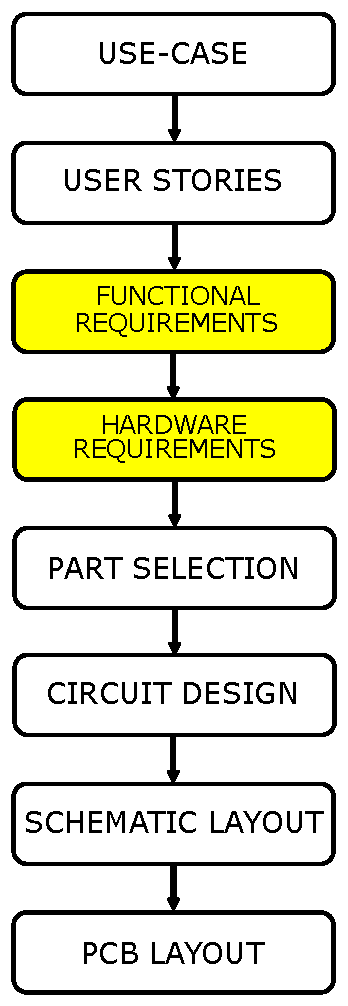
\includegraphics[width=0.5\linewidth]{Figures/requirements.pdf}\centering
%	\label{fig:requirements}
%\end{figure}

%----------------------------------------------------------------------------------------

\subsection{Power Control Requirements}
The following requirements are related to the Power Control schematic, which can be found in \autoref{chap:batt}.
\begin{enumerate}
\item Powered with a single-cell LiFePO4 battery
\item Controlled output from single-cell LiFePO4 battery 
\item Disabling the power supply to 4G LTE Modem
\item Disabling the power supply to FPGA and dependent components via GPIO line of FPGA
\item Enabling the 3.3V power supply to FPGA and dependent components by employing momentary switch
\item Enabling the 3.3V power supply to FPGA and dependent components by an interrupt signal from the 4G modem (also see \autoref{chap:modem})
\item Enabling the 3.3V power supply to FPGA and dependent components by an alarm signal from a Real-Time Clock (also see \autoref{chap:RTC})
\item Microphone input from headphone and internal microphone can be physically disabled with a switch 
\item Disabling the 3.3V supply to the WiFi module via a signal from the FPGA board
\item Power Indication LED for 4G LTE module
\item Power Indication LED for FPGA board 
\item Power Indication LED for WiFi board
\item 3.3V supply to the 4G module controlled via a signal from the FPGA, but only if physical switch is set to allow 4G module to be powered
\end{enumerate}

\subsection{Connectors and Switches}
\begin{enumerate}
\item 25-pin DSUB connector for SX-64 keyboard 
\item VGA connector providing video output with at least 4-bits colour depth per channel (see \autoref{chap:VGA})
\item WiFi module interconnection with the FPGA via UART interface
\item UART, I2C, input and output PCM audio interfaces and ADC interfaces between 4G module and the FPGA board (see \autoref{chap:modem} and \autoref{chap:FPGA})
\item 2 x 9-pin C64 joystick ports
\item Four momentary-action user buttons 
\item Wireless co-existence interface between WiFi and 4G modules 
\item Micro-USB connector and charger
\end{enumerate}

\subsection{Peripheral Devices}
\begin{enumerate}
\item Real-Time Clock IC to maintain time and date when switched off, and to set alarms (see \autoref{chap:RTC})
\item 4 Microphones (see \autoref{chap:mics})
\item Proximity sensor for blanking screen during calls (see \autoref{chap:prox})
\item Ambient light sensor 
\item Speaker for audio output (see \autoref{chap:audio})
\item Headphone jack (see \autoref{chap:audio})
\item Audio output to speaker and headphone jack can be independently controlled (see \autoref{chap:audio} and \autoref{chap:audio2})
\item Micro SD card slot to be connected to FPGA board (see \autoref{chap:SIM})
\item LCD panel connected via digital VGA interface with at least 6 bits colour depth per channel (see \autoref{chap:LCD})
\item LCD capacitive touch digitiser via I2C to FPGA board (see \autoref{chap:touch})
\item Accelerometer connected via I2C to FPGA board (see \autoref{chap:a})
\item 4 SIM card sockets connected to 4G module via SIM MUX ICs (see \autoref{chap:SIM})
\end{enumerate}

%----------------------------------------------------------------------------------------



